\section{Capacitive proximity sensing applications}
\subsection{A brief history of capacitive proximity sensing}
\begin{figure}[h]
\centering
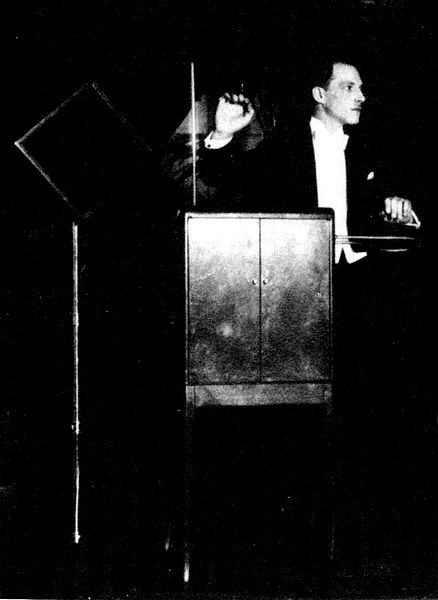
\includegraphics[width=0.4\textwidth]{images/leon_theremin.jpg}
\caption{Leon Theremin playing his epnoymous electronic musical instrument \cite{Glinsky2000}}
\label{fig:leon_theremin}
\end{figure}
In the last decades of the 19th and the beginning of the 20th century a considerable number of inventors and scientists performed research on the application of electric systems, sparking innovations such as electric lighting, electric motors, telegraphy and radio communication. Lev Sergeyevich Termen or Léon Theremin in the American naming was a Russian inventor most famous for designing the theremin. This early electronic musical instrument could be played without touch. One hand is controlling the pitch and the other the volume by changing the distance to an antenna. Initially designed as a motion detector, this device is transferring the influence of the human body on an oscillating electric field to an audible sound \cite{Glinsky2000}. 

Electric field imaging was a research focus at the MIT in the 1990s. A research group in the Media Lab division including Joseph A. Paradiso, Thomas G. Zimmerman, Joshua R. Smith designed various sensing devices and evaluated various applications in HCI \cite{Zimmerman1995}\cite{Smith1999a}.
- NEC passenger seat
- Paradiso/Smith
- Wimmer
- Touché
- Swallowing
- Hamburg Gruppe
- Finnland Anwendungen
